\chapter[Diseño de Solución]{Diseño de Solución}
\label{cp:design}

\parindent0pt

- La importancia de esta etapa esta en que si te la saltas luego el desarrollo se vuelve más complicado y propenso a errores, gaps, inconsistencias.

------------

En la fase de modelado de requerimientos se definieron las bases del sistema, estableciendo sus funcionalidades y características que el prototipo debe cumplir. Este capítulo aborda la etapa de diseño de solución, que es una transición entre la especificación de lo que el sistema debe hacer y el cómo se construirá, transformando los requisitos abstractos en una arquitectura concreta y un plan de implementación. El diseño permite obtener una visión integral del sistema antes de iniciar la implementación, lo que facilita la identificación de dependencias e interfaces y asegura que todos los componentes y módulos interactúen de manera coherente. Este proceso de planificación anticipada reduce la probabilidad de encontrar inconsistencias, fallas de lógica o funcionalidades indefinidas durante las fases de desarrollo y pruebas.

El diseño de la solución, en el marco del modelo en V, se aborda en dos etapas: primero se realiza el diseño de arquitectura y luego el diseño de componentes. Cada una de estas etapas se enfoca en un nivel de abstracción distinto del sistema. El diseño de arquitectura comprende la defición de la estructura general del sistema a través de módulos, mientras que el diseño de componentes se ocupa de los detalles internos de cada módulo.

En la primer etapa, diseño de arquitectura, el sistema se divide en subsistemas o módulos lógicos, y se definen sus interacciones, las responsabilidades de cada uno y las tecnologías subyacentes. Este enfoque permite establecer las bases del sistema, abarcando tanto los requerimientos funcionales como los no funcionales. Las decisiones de diseño tomadas en esta etapa se validan posteriormente mediante pruebas de sistema, las cuales se encargan de verificar que todos los módulos trabajen conjuntamente y que el sistema de forma integral satisfaga los requerimientos especificados.

Por otro lado, la segunda etapa es el diseño de componentes, donde se profundiza en los detalles de la arquitectura interna de cada módulo. Esto incluye la especificación de clases, interfaces, flujos de datos y la organización de la lógica de negocio. Los requerimientos funcionales, guiados por las historias de usuario, se traducen en documentos de arquitectura de software específicos que posteriormente se implementan en la fase de codificación. Las decisiones de diseño tomadas en esta etapa se verifican a través de las pruebas de integración, que aseguran que los componentes individuales interactúen de forma correcta entre sí.

Los requerimientos funcionales, definidos en el capítulo anterior, son el fundamento para el diseño de la solución y se utilizan en esta etapa a través de las historias de usuario, que guían el diseño de los módulos y componentes. De manera complementaria, los requerimientos no funcionales también se contemplan en la fase de diseño, particularmente en el diseño de arquitectura, donde se establecen las bases para garantizar atributos como la seguridad, el rendimiento y la escalabilidad, incluso si no están directamente asociados a una historia de usuario.

A continuación, se explicará cada una de las etapas del diseño de solución, comenzando con el diseño de arquitectura en la sección \ref{sec:module-design}, seguido por el diseño de componentes en la sección \ref{sec:components-design}.

\section{Diseño de Arquitectura}
\label{sec:module-design}

- Esta etapa se centra en tal cosa y es la primera, su entrada son los requerimientos, su salida es la arquitectura del sistema, que comprende módulos, interacciones y tecnologías.
- Contar sobre la etapa de pruebas correspondiente del otro lado.
- Criterios para separar módulos y definir las interfaces (basicamente usamos los estandares de la industria para apps webs de modo que en el futuro sea extensible, mantenible e integrable con otras fuentes de datos como iot en los procesos productivos).
- Empezar a contar: Primero armé la arquitectura del sistema, separando en bloques frontend/api/datos. 
- Contar que decidí separar los módulos segun rol y los compartidos aparte por el acoplamiento y separación de responsabilidades.
- Contar para cada módulo la comparación y elección de tecnologías. 
- Contar la comparación de blockchains y mencionar el apendice, justificar la elección de blockchain.
- Explicar también las interfaces entre módulos (API rest en gral), pero si usé alguna librería para estas interfaces explicar cuál.
- Contar sobre las combinación de blockchain y sql, y cómo se relacionan los datos de la blockchain con los datos de la base de datos sql. Esto con fines de escalabilidad y rendimiento. No se uso the graph por el alcance del trabajo, era un overkill para el tamaño del prototipo.
- incluir un diagrama de despliegue que ilustre dónde se ejecutan los diferentes componentes (servidor web, base de datos, nodo de blockchain, etc.). Esto da una visión de cómo se vería el sistema en el entorno de producción.

--------

La fase de diseño de arquitectura representa el primer paso en la traducción de los requerimientos del sistema hacia un sistema de software funcional. El diseño permite una visión global de la solución, asegurando que todos los componentes y módulos trabajen juntos de manera coherente previo a la implementación. A partir de los requerimientos previamente definidos, se establece un marco de trabajo de alto nivel que estructura la solución en componentes lógicos, delineando sus responsabilidades, las interacciones entre ellos y las tecnologías que los soportan. La salida de esta etapa es la arquitectura del sistema, la cual servirá de base para las decisiones de diseño a un nivel más granular. En el contexto del modelo en V, las decisiones tomadas en esta etapa se validan en la fase de pruebas de sistema, donde se verifica que la arquitectura en su conjunto cumple con las especificaciones definidas en los requerimientos funcionales y no funcionales del sistema.
\begin{figure}[!htpb]
    \centering
    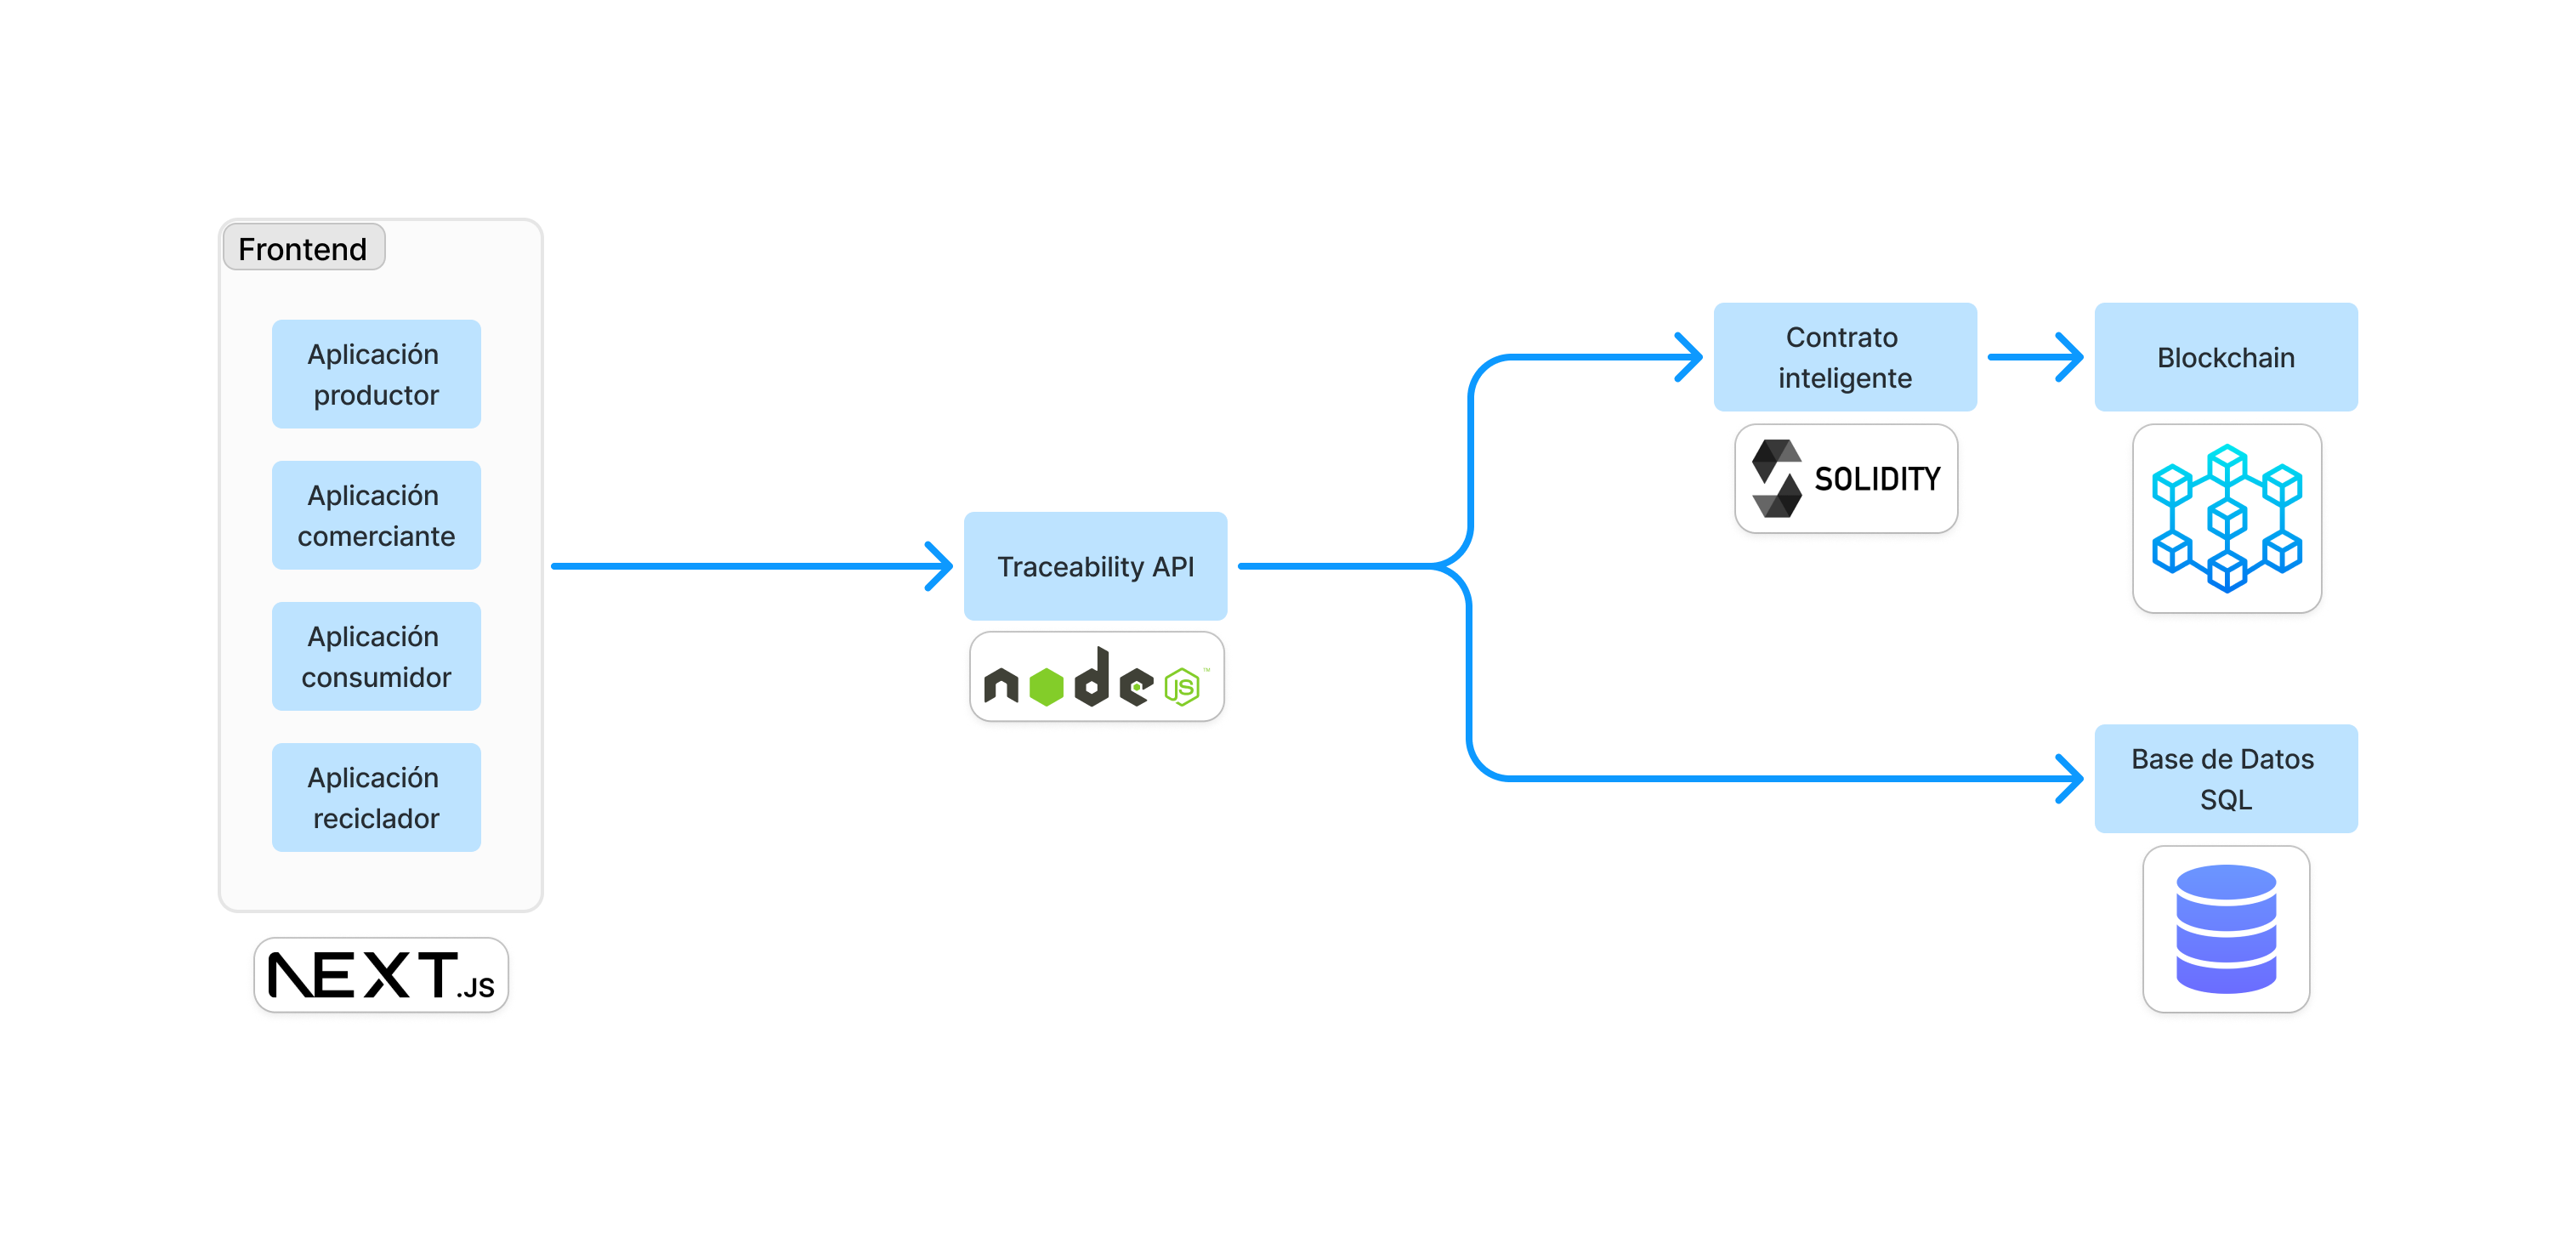
\includegraphics[width=0.8\textwidth]{Figures/software-architecture.png}
    \caption{Arquitectura del sistema}
    \label{fig:software-architecture}
\end{figure}

Para el prototipo tecnológico de trazabilidad de vidrio basado en blockchain, la arquitectura del sistema se concibió siguiendo un enfoque de tres capas lógicas para asegurar una clara separación de responsabilidades y modularidad. Este patrón, común en el desarrollo de aplicaciones web, permite que cada capa se desarrolle, mantenga y escale de forma independiente. La arquitectura se compone de la capa de presentación (frontend), la capa de lógica de negocio (backend) y la capa de datos (blockchain y base de datos relacional). La comunicación entre estas capas se define a través de interfaces estandarizadas, lo que promueve una baja dependencia y puede facilitar futuras extensiones e integraciones, por ejemplo, con sistemas de gestión externos o con dispositivos de Internet de las Cosas (IoT) para automatizar la captura de datos en los procesos productivos.

A su vez, dentro de cada capa del sistema, es necesario definir un criterio para la delimitación de los módulos lógicos dentro de la misma capa. El criterio aplicado en este trabajo se basa en el principio de cohesión funcional, el cual plantea agrupar las funcionalidades y responsabilidades del sistema a partir de cada rol de usuario identificado. Siguiendo este criterio, para este trabajo se definió implementar un módulo específico para cada actor (productor primario, productor secundario, consumidor y centro de reciclaje), así como módulos compartidos para la lógica de negocio transversal, como la autenticación de usuarios o trazabilidad de envases de vidrio. Esta división de responsabilidades reduce el acoplamiento entre los módulos y simplifica el mantenimiento del sistema, en el caso de requerir cambios o actualizaciones en el futuro.

Luego de definir las capas que componen la arquitectura del sistema, es posible proceder a seleccionar las tecnologías más adecuadas para cada uno de los módulos definidos. La elección de tecnologías para cada capa busca satisfacer una serie de criterios técnicos y de negocio, incluyendo la compatibilidad con otras tecnologías, el rendimiento, la escalabilidad y el soporte de la comunidad. 

A continuación, se describen las tecnologías seleccionadas, los patrones de diseño aplicados y las decisiones arquitectónicas tomadas para cada capa del sistema. Comenzando por la capa de datos, se explicará la arquitectura desde adentro hacia afuera, siguiendo el flujo de datos desde su almacenamiento hasta la presentación al usuario final.

\subsection{Capa de Datos}

La capa de datos constituye el cimiento de todo sistema de software. Se encarga de la persistencia, gestión y recuperación de toda la información del sistema. 

Las bases de datos relacionales son el tipo de base de datos más utilizado actualmente para gestionar información estructurada. Los datos se organizan en tablas, con filas y columnas, y se pueden establecer relaciones entre las distintas tablas mediante claves únicas. Cada columna tiene tiene un nombre y un tipo de dato asociado, mientras que cada fila representa un registro único dentro de la tabla y su contenido debe cumplir con el tipo de dato definido para cada columna. Por ejemplo, se podría definir una tabla "Usuario", para almacenar información sobre los usuarios del sistema, incluyendo columnas como "nombre" de tipo texto, "correo electrónico" de tipo texto y "fecha de registro" de tipo fecha, entre otras columnas. Cada fila en esta tabla representaría un usuario específico, con su nombre, correo electrónico y la fecha en que se registró en el sistema, entre otros datos. Las principales ventajas de las bases de datos relacionales radican en su capacidad para garantizar la uniformidad de los datos a través de esquemas definidos para cada tabla, así como la facilidad para realizar consultas y análisis complejos de manera eficiente. Sin embargo, su naturaleza centralizada las hace susceptibles a manipulaciones manuales difíciles de detectar, lo que justifica la necesidad de una tecnología complementaria, como la blockchain, para registrar información que requiere garantías de integridad.

En este prototipo, la tecnología blockchain resulta apropiada para registrar la información clave del sistema, que requiere inmutabilidad y transparencia para fomentar la confianza entre los distintos actores. Ejemplos de este tipo de información puede ser la propiedad de los lotes de envases vidrio o la trazabilidad de los envases reciclados. Por este motivo, se tomó la decisión estratégica de combinar la blockchain con una base de datos relacional con el objetivo de resolver la necesidad de equilibrio entre la seguridad y la transparencia, con el rendimiento y la escalabilidad. La blockchain, por su naturaleza, provee una fuente de información segura y transparente, pero puede presentar limitaciones en cuanto a la velocidad de las transacciones y el volumen de datos que permite consultar eficientemente. Para abordar estas limitaciones, es que se decidió utilizar la blockchain como base de datos principal del sistema, mientras que se decidió utilizar una base de datos relacional complementaria para almacenar datos auxiliares e indexar los datos de acceso frecuente, como los perfiles de usuario, los metadatos de los lotes (id, propietario, estado, etc.) y otros datos de soporte que no requieren inmutabilidad. La relación entre ambas fuentes de datos se maneja mediante identificadores únicos que se almacenan en la blockchain, sirviendo como una referencia a los datos detallados en la base de datos relacional. La capa backend es responsable de mantener la consistencia entre ambas fuentes de información (blockchain y base de datos relacional) a la hora de persistir nueva información o actualizar información existente. Este enfoque híbrido permite proveer una recuperación de información ágil y una experiencia de usuario fluida sin poner en compromiso la integridad de los datos sensibles.

Luego de definir la estrategia de almacenamiento y gestión de datos, es posible proceder a seleccionar las tecnologías específicas que se utilizarán, tanto para la base de datos relacional como para la plataforma blockchain, ya que existen múltiples opciones en el mercado.

En el caso de la base de datos relacional, se optó por el uso de MariaDB \footnote{https://mariadb.org/documentation/}, una base de datos de código abierto elegida por su sencillez y familiaridad, ya que el uso que se le dará en este trabajo es complementario y no hace falta utilizar una alternativa más compleja. MariaDB cuenta con un amplio soporte, librerías y documentación disponible para conectarse a ella de forma estandarizada desde cualquier lenguaje o framework utilizado en la capa backend.

Por otro lado, para la tecnología blockchain, la elección de una plataforma adecuada puede determinar la complejidad y tiempo de implementación del sistema.  La tecnología blockchain no se implementa desde cero, sino que se utilizan plataformas ya desarrolladas y probadas que ofrecen características y funcionalidades específicas. Estas plataformas, conocidas como protocolos blockchain, varían en aspectos como su mecanismo de consenso, lenguaje de programación y comunidad de desarrolladores. Para este trabajo, se analizaron cinco de las plataformas líderes en la industria para su análisis y comparación: Hyperledger Fabric, Ethereum, Polkadot, VeChain y Cardano. Estas plataformas se seleccionaron por su relevancia y características técnicas, evaluando su idoneidad para el caso de uso específico de trazabilidad en la cadena de suministro del vidrio.

\textbf{Hyperledger Fabric} \footnote{https://hlf.readthedocs.io/en/latest/}
es una plataforma de código abierto diseñada para uso empresarial, que forma parte de la Fundación Linux \cite{androulaki2018hyperledger}. Se caracteriza por su arquitectura modular y configurable, ideal para una amplia gama de casos de uso en la industria. A diferencia de las redes públicas, es una plataforma permisionada, lo que significa que los participantes se conocen y confían entre sí. Admite contratos inteligentes en lenguajes de programación comunes como Java y Node.js, lo que reduce la curva de aprendizaje. Hyperledger no requiere una criptomoneda nativa, lo que elimina ciertos riesgos de ataque y permite que la plataforma se implemente con costos operativos similares a los de cualquier otro sistema distribuido.

\textbf{Ethereum} \footnote{https://ethereum.org/en/developers/docs/}
es una plataforma de código abierto y pública que permite a los desarrolladores crear contratos inteligentes y aplicaciones descentralizadas (dApps). Se considera una computadora mundial descentralizada, alimentada por su criptomoneda nativa, Ether. Ethereum fue pionera en la creación de contratos inteligentes y ha mantenido un liderazgo en la industria desde su lanzamiento en 2015. Los contratos se escriben en Solidity, un lenguaje de programación de dominio específico que se ejecuta en la red de Ethereum. Aunque se lanzó con un protocolo de consenso de Prueba de Trabajo (PoW), la plataforma ha migrado a la Prueba de Participación (PoS) para mejorar su eficiencia energética y escalabilidad.

\textbf{Polkadot} \footnote{https://docs.polkadot.com/}
es una plataforma de código abierto que busca facilitar la interoperabilidad entre diferentes blockchains. Su objetivo es crear una red escalable y segura que pueda soportar una amplia gama de aplicaciones descentralizadas. Su arquitectura se basa en una cadena principal (Relay Chain) y múltiples cadenas que se conectan a ella (parachains), permitiendo que las blockchains se comuniquen entre sí de manera eficiente a través de la Relay Chain. Utiliza un protocolo de consenso derivado de PoS, llamado Nominated Proof of Stake (NPoS) y su criptomoneda nativa es DOT. Las aplicaciones se desarrollan con Substrate, un framework modular escrito en Rust, que también es compatible con contratos inteligentes escritos en Solidity.

\textbf{VeChain} \footnote{https://docs.vechain.org/}
es una plataforma de código abierto dedicada específicamente a la trazabilidad y la autenticación de productos en la cadena de suministro. Combina tecnología blockchain con identificación por radiofrecuencia (RFID) e Internet de las cosas (IoT) para rastrear productos desde la producción hasta el consumidor final. Es una plataforma permisionada, donde los participantes se conocen y confían mutuamente, lo que permite una mayor privacidad y confidencialidad. Utiliza una arquitectura de dos tokens (VET y VTHO) y un protocolo de consenso de Prueba de Autoridad (PoA). Al ser compatible con Solidity, facilita la migración de aplicaciones existentes de Ethereum.

\textbf{Cardano} \footnote{https://docs.cardano.org/}
es una plataforma de blockchain de código abierto que se enfoca en la creación de una red escalable, segura y sostenible. Se distingue por su enfoque científico y riguroso, utilizando evidencia formal y revisión por pares para garantizar la seguridad y confiabilidad de la plataforma. Para programar aplicaciones se utiliza el lenguaje de programación funcional Haskell, que permite la verificación formal de los contratos inteligentes. También se pueden desarrollar contratos utilizando Plutus, un lenguaje de dominio específico basado en Haskell. La red utiliza un protocolo de consenso PoS y su criptomoneda nativa es ADA.

En la Tabla \ref{tab:blockchain-comparison}, se presenta un resumen comparativo de los protocolos blockchain analizados, destacando los aspectos relevantes de cada uno para la selección del más adecuado para este trabajo.

\begin{table}[!tb]
	\centering
	\begin{tabular}{|c|c|c|c|c|c|}
	\hline
	\textbf{Tecnología} & \textbf{Hyperledger} & \textbf{Ethereum} & \textbf{Polkadot} & \textbf{VeChain} & \textbf{Cardano} \\ \hline
	\\ \hline
	Consenso & Flexible & PoW - PoS & NPoS & PoA & PoS \\ \hline
	Lenguaje & Java, Go, Node.js & Solidity & Rust, Solidity & Solidity & Haskell \\ \hline
	Interoperabilidad & Limitada & Limitada & Alta & Limitada & Limitada \\ \hline
	Adopción & Alta & Muy alta & Media & Media & Media \\ \hline
	Comunidad & Grande & Grande & Grande & Mediana & Grande \\ \hline
\end{tabular}
\caption{Comparación de plataformas blockchain}
\label{tab:blockchain-comparison}
\end{table}

Luego de realizar el análisis comparativo entre protocolos blockchain, se llega a la determinación de que Ethereum resulta ser la tecnología más adecuada para este trabajo por múltiples razones. En primer lugar, su naturaleza pública está alineada con el objetivo del proyecto, ya que permite a cualquier persona unirse a la red y verificar el estado de la cadena de forma transparente, sin necesidad de permisos, como puede ocurrir en las plataformas permisionadas como Hyperledger. A su vez, otro factor influyente en esta elección es la adopción del mecanismo de consenso PoS en la red Ethereum, que es más eficiente energéticamente que PoW, de modo que se alinea directamente con los objetivos de sostenibilidad ambiental del proyecto. Además, Ethereum posee la mayor comunidad de desarrolladores entre las plataformas analizadas y una alta adopción en la industria, lo que garantiza un soporte continuo y una amplia gama de herramientas y recursos a su disposición. Su lenguaje de programación, Solidity, es de alto nivel y fácil de aprender en comparación a lenguajes como Rust y Haskell, permitiendo la creación de aplicaciones complejas de manera eficiente. Finalmente, existe una amplia variedad de herramientas que permiten conectar otras tecnologías y sistemas con Ethereum, facilitando la integración con la base de datos relacional y la capa backend del sistema.

Sin embargo, Ethereum presenta algunas desventajas, como los altos costos de transacción y alta latencia de red, que pueden afectar la experiencia del usuario y la viabilidad económica del sistema. Afortunadamente, en la actualidad existen múltiples soluciones para mitigar estos problemas. En particular, para mitigar los altos costos y la latencia de la red de Ethereum para esta aplicación de trazabilidad que puede alcanzar un volumen de datos considerable, se decidió realizar el despliegue de los contratos en una solución de capa 2 de Ethereum. Este tipo de solución en capas permite procesar las transacciones fuera de la cadena principal para luego sincronizarlas, lo que reduce costos y aumenta la escalabilidad, sin comprometer la seguridad ni la integridad de los datos de la blockchain. A su vez, se eligió hacer uso del framework Hardhat para el desarrollo y despliegue de los contratos inteligentes, ya que es una herramienta ampliamente adoptada que facilita la implementación y ejecución de pruebas unitarias y de integración sobre contratos inteligentes en Solidity.

\subsection{Capa Backend}

La capa de lógica de negocio, generalmente conocida como \textit{backend} o \textit{API}, actúa como el cerebro del sistema. Su propósito principal es implementar y ejecutar las reglas de negocio del sistema, orquestar la interacción entre las distintas capas (capa frontend y capa de datos), y exponer una interfaz estandarizada a través de la cual otros componentes puedan interactuar con la funcionalidad del sistema, sin depender de su implementación interna.

Para este prototipo, se ha optado por implementar una arquitectura desacoplada, donde la capa de presentación (frontend) y la capa de lógica de negocio se desarrollan de forma independiente. Este tipo de arquitectura desacoplada resulta necesaria para un sistema de las características de este trabajo. A diferencia de una arquitectura monolítica, este enfoque promueve la modularidad y la escalabilidad, permitiendo que la interfaz de usuario pueda evolucionar o ser reemplazada sin afectar la lógica de negocio central de la aplicación. Este diseño responde directamente al requerimiento no funcional de interoperabilidad (RNF-05), ya que la API de trazabilidad está pensado para ser el punto de integración principal no solo para el frontend del prototipo, sino también para sistemas de gestión preexistentes, dispositivos IoT y otras aplicaciones de terceros que pudieran surgir en el futuro para la trazabilidad de procesos de la cadena de suministro y reciclaje de los envases de vidrio.

Para la implementación de la capa backend se tomó la decisión de utilizar la tecnología Node.js \footnote{https://nodejs.org/es}, un entorno de ejecución del lenguaje Javascript que permite crear servidores, aplicaciones web, herramientas de línea de comandos y \textit{scripts}. A su vez, JavaScript es un lenguaje de programación de alto nivel, interpretado y dinámico, que es ampliamente conocido y utilizado para el desarrollo web tanto en frontend como en backend. Su curva de aprendizaje es relativamente baja y es el lenguaje que se utiliza para dar dinamismo a las páginas web. Sin embargo, su uso también se ha extendido al lado del servidor gracias a entornos de ejecución como Node.js, lo que ha permitido a los desarrolladores crear aplicaciones web completas utilizando un único lenguaje de programación. Su popularidad y amplia adopción en la industria, se deben a su flexibilidad y a la gran cantidad de librerías y frameworks que se han desarrollado para este lenguaje, que permiten construir tanto aplicaciones web simples, como sistemas complejos y escalables.

Existen múltiples motivos que justifican la elección del entorno Node.js para el desarrollo de la capa backend de este trabajo. En primer lugar, considerando el alcance limitado del trabajo, Javascript resulta ser un lenguaje propicio debido a su baja curva de aprendizaje y su flexibilidad para ser utilizado tanto en la capa backend como en la capa frontend, lo que facilita el proceso de desarrollo al permitir que el mismo desarrollador trabaje en ambas capas sin necesidad de cambiar de lenguaje. Existen múltiples lenguajes y frameworks ampliamente utilizados en la industria para desarrollar la capa backend de aplicaciones web, como Java con Spring Boot, Python con Django o Flask y Ruby on Rails, pero la posibilidad de utilizar el mismo lenguaje tanto en frontend como en backend, simplifica el proceso de desarrollo en equipos pequeños o unipersonales y ayuda a facilitar el mantenimiento del código en el futuro. A su vez, Node.js ofrece una excelente soporte para la interacción con la red de Ethereum, mediante una serie de librerías ampliamente adoptadas y probadas en la comunidad, como pueden ser Ethers.js y Web3.js. Por último, la amplia adopción de Node.js en la industria y la disponibilidad de herramientas para pruebas unitarias facilitan el desarrollo y el mantenimiento del sistema. 

Por otro lado, la comunicación del backend con las demás capas del sistema debe implementarse a través de interfaces bien definidas. Con la capa de presentación, el backend se comunica mediante una API RESTful. El estándar REST (Representational State Transfer) define una arquitectura para la comunicación entre sistemas que se basa en el uso del protocolo HTTP para intercambiar información sin mantener un estado entre intercambios. Una API RESTful utiliza los métodos estándar de HTTP (como GET, POST, PUT, DELETE) para realizar operaciones sobre los recursos del sistema, y el formato JSON para el intercambio de datos. Por ejemplo, el frontend del sistema podría enviar una solicitud GET a la API para solicitar la lista de envases de vidrio producidos por cierto productor primario. En este caso, el backend respondería con la información solicitada en formato JSON y el frontend podría utilizar esta información para actualizar la interfaz de usuario, mostrando el listado de los envases de vidrio correspondientes al usuario.

Dentro del entorno de Node.js, existen múltiples librerías y frameworks que facilitan el desarrollo de APIs REST. La opción más popular y ampliamente adoptada es Express.js \footnote{https://expressjs.com/}, un framework minimalista y flexible que proporciona las utilidades esenciales para la construcción de APIs RESTful. Entre sus principales ventajas se encuentran su simplicidad, flexibilidad y extensibilidad. Gracias a estas características, Express.js es utilizado para construir API REST directamente, pero también ha sido utilizado como base de múltiples frameworks de desarrollo de APIs RESTful más complejos, como Nest.js, Sails.js y Sails.js, entre otros. Estos frameworks extienden las funcionalidades de Express.js y facilitan el desarrollo de APIs RESTful en Node.js, añadiendo funcionalidades adicionales que mejoran la mantenibilidad y escalabilidad de las APIs RESTful. Sin embargo, estos frameworks suelen imponer una estructura más rígida y una curva de aprendizaje más pronunciada que Express.js. Por este motivo, se decidió utilizar Express.js como base para el desarrollo de la API del sistema, ya que no impone restricciones adicionales sobre el modelo arquitectónico y permite una implementación eficiente y escalable, sin sacrificar la flexibilidad necesaria para adaptarse a los requerimientos específicos del sistema.

Finalmente, para la interacción con la capa de datos, el backend se conecta a la base de datos relacional mediante librerías de conexión estandarizadas y a la blockchain a través de librerías de interacción con contratos inteligentes, lo que permite un acceso unificado a los datos, abstrayendo la complejidad de cada fuente de datos y proporcionando una interfaz coherente para la capa frontend del sistema.

Capa de Presentación (Frontend)
La capa de presentación, conocida habitualmente como \textit{frontend}, es la interfaz de usuario web que permite a los distintos actores de la cadena de suministro interactuar con el sistema de trazabilidad del vidrio. Su objetivo es traducir la lógica de negocio y los datos que provienen de la API en una experiencia visual y funcional, permitiendo que los usuarios interactúen con el prototipo de manera intuitiva. El frontend es la cara visible del sistema completo.

Para este prototipo, se tomó la decisión de implementar de forma desacoplada la interfaz de la lógica de negocio, con el objetivo de reforzar la mantenibilidad y flexibilidad del sistema. Esta separación es propicia para que la interfaz de usuario pueda evolucionar de manera independiente de la lógica, adaptándose a nuevas necesidades, experiencias de usuario o tecnologías sin afectar el funcionamiento del sistema. Con este esquema, es factible que en un futuro, cada actor de la cadena tenga acceso a una interfaz a medida de sus necesidades. Por ejemplo, para un productor de envases de vidrio, se podría desarrollar una aplicación de escritorio con métricas de negocio sobre su producción y venta, mientras que para los consumidores, se podría crear una aplicación móvil que muestre puntos de reciclaje y ofrezca incentivos por reciclar. Aunque el prototipo desarrollado para este trabajo final presenta una interfaz web unificada para todos los actores, el diseño modular facilita la creación de estas aplicaciones independientes en el futuro.

La elección tecnológica para esta capa estuvo focalizada en encontrar frameworks y librerías que promuevan la modularidad y la eficiencia durante el desarrollo. En primer lugar, se determinó utilizar React \footnote{https://es.react.dev/} como librería base para la construcción de la interfaz, debido a su modelo de desarrollo basado en componentes, que promueve la reutilización de código. A su vez, para potenciar React, se optó por hacer uso del framework Next.js \footnote{https://nextjs.org/docs}, que agrega funcionalidades extra a React para facilitar aún más el desarrollo de aplicaciones web modulares y de alto rendimiento, combinando técnicas como generación de sitios estáticos y renderizado en el servidor. Por otro lado, para el diseño de las interfaces web se utiliza el lenguaje de estilado CSS, que en este prototipo se complementó con el uso de la librería Tailwind CSS \footnote{https://tailwindcss.com/} que promueve una estética moderna y una sintaxis simplificada dentro del código.

La comunicación del frontend con el backend se realiza exclusivamente a través de llamadas a la API RESTful. La interfaz no contiene la lógica de negocio, sino que actúa como un cliente ligero que envía datos al backend (por ejemplo, al registrar un nuevo lote) y recibe la respuesta, la cual es luego presentada al usuario. Este modelo garantiza que el frontend se enfoque en la interacción y la visualización, mientras la lógica crítica reside en el backend. Debido a que el frontend se enfoca únicamente en la visualización de información, es necesario implementar un sistema de autenticación y autorización unificado entre frontend y backend que permita a cada usuario visualizar e interactuar únicamente con las funcionalidades propias de su rol. Por este motivo, para gestionar la autenticación de usuarios este proyecto, se determinó hacer uso del servicio Firebase Authentication, que gestiona la autenticación de usuarios e implementa de forma abstracta el estándar de autorización OAuth 2.0, asegurando que solo los actores con los permisos adecuados puedan acceder a cada recurso del sistema.

Luego de definir la arquitectura de la aplicación web, incluyendo la definición de capas, la comunicación entre ellas y los lenguajes de programación a utilizarse, es posible comenzar con la etapa de diseño de componentes. En esta segunda etapa de diseño, se define la arquitectura interna de cada capa o módulo definido en la etapa anterior. En la próxima sección, se detallará el diseño de componentes de este sistema, que abarca la estructura interna del frontend, la API y la capa de datos.

\section{Diseño de Componentes}
\label{sec:components-design}

- Esta etapa es la segunda y se centra en tal cosa, su entrada son los módulos y requerimientos y su salida es la arquitectura de componentes, que comprende estructura de pantallas, apis y contratos.



- Contar que elegi arch de módulos MVC en front, por qué y mostrar la división de funcionalidades por pantalla. Explicar que es MVC pero conciso y que se enfoque en por qué fue la elección correcta para esto, en lugar de ser una lección teórica.
- Contar en el front que también se eligió el sistema de diseño y paleta de colores, íconos, disposición del sistema y personalidad. Se decidió que sea una plataforma web, no mobile.
- Contar que elegí clean arch en back, por qué y mostrar la división de funcionalidades por módulo. Mostrar la división de dominio. Explicar que es clean arch pero conciso y que se enfoque en por qué fue la elección correcta para esto, en lugar de ser una lección teórica. Api mencionar los endpoints de cada modulo o la lista de modulos almenos con su dominio.
- Contar cómo armé la arquitectura de contratos en la blockchain y el modelo de datos en sql para un trackeo eficiente, confiable y no redundante de información. Mostrar los DER y reexplicar en detalle su interacción. Contar qué cubre cada contrato y cada tabla.
- Explicar como el repository+handler unifica ambas cosas


- Transicionar al siguiente cap. Que es la implementación, que es la etapa de desarrollo de la solución, donde se implementan los módulos y componentes diseñados en las etapas anteriores. Que haber hecho este diseño permite una implementación más fluida y organizada, ya que se cuenta con una guía clara de cómo deben interactuar los diferentes componentes y módulos.

------ 

Esta etapa toma como entrada los requerimientos del sistema y la arquitectura de módulos, y su salida es un conjunto de especificaciones detalladas que guiarán la implementación, asegurando la cohesión interna de cada módulo y su correcta interacción. Las decisiones de diseño tomadas en esta etapa se verifican en la fase de pruebas de integración, que valida la comunicación entre los componentes del sistema.

La segunda etapa de diseño, el diseño de componentes, se ocupa de detallar la arquitectura interna de los módulos definidos en la fase anterior. Su propósito es traducir la arquitectura de alto nivel en un plan de construcción específico, que incluye la estructura de la interfaz de usuario, la arquitectura de la API y el modelo de datos. Esta fase toma como entrada los requerimientos del sistema y la arquitectura de módulos, y su salida es un conjunto de especificaciones detalladas que guiarán la implementación, asegurando la cohesión interna de cada módulo y su correcta interacción. Las decisiones de diseño tomadas en esta etapa se verifican en la fase de **pruebas de integración**, que valida la comunicación entre los componentes del sistema.

### Arquitectura de la Interfaz de Usuario

La interfaz de usuario se diseñó como una aplicación web de página única (SPA), lo que permite una experiencia de usuario fluida y reactiva, sin recargar la página en cada interacción. Se optó por una plataforma web en lugar de una aplicación móvil nativa para maximizar la accesibilidad y reducir la complejidad de desarrollo y mantenimiento, lo que es congruente con el alcance del prototipo. El diseño se estructuró siguiendo una arquitectura basada en componentes, inspirada en el patrón de desarrollo dirigido por componentes. Este enfoque permite la creación de elementos de interfaz reutilizables, modulares e independientes, que se agrupan en una biblioteca. Esta metodología facilita la construcción rápida y consistente de las vistas de la aplicación y mejora la mantenibilidad del código a largo plazo, ya que los componentes pueden ser actualizados sin afectar otras partes del sistema.

La estructura de la interfaz de usuario se organizó por módulos funcionales y por rol de usuario, lo que se alinea con la división de responsabilidades establecida en el diseño de arquitectura. Por ejemplo, se definieron vistas específicas para el registro y gestión de lotes por parte de los productores, así como una interfaz de consulta para los consumidores. Adicionalmente, se creó un sistema de diseño que incluye la paleta de colores, la tipografía y la iconografía, con el fin de proporcionar una identidad visual consistente y una experiencia de usuario unificada en toda la plataforma.

### Arquitectura de la Capa de Lógica de Negocio (API)

Para la capa de la API, se adoptó la **Arquitectura Limpia** (Clean Architecture), un patrón de diseño que prioriza la separación de las reglas de negocio del resto de las dependencias. Esta elección se justifica por su capacidad para generar un sistema con un alto grado de desacoplamiento, lo que se traduce en una mayor testabilidad, mantenibilidad y flexibilidad. En este modelo, la lógica de negocio se ubica en el núcleo de la arquitectura, rodeada por capas que se encargan de la infraestructura, las interfaces de usuario y las bases de datos. Esta estructura permite que la lógica de negocio no se vea afectada por cambios en las tecnologías de implementación, como la base de datos o la interfaz de usuario, lo que prolonga la vida útil del sistema.

La arquitectura de la API se dividió en módulos de dominio, con un enfoque en la lógica de negocio que encapsula cada funcionalidad del sistema. Por ejemplo, se definieron dominios para la gestión de usuarios, la trazabilidad de lotes y las transacciones. Cada uno de estos dominios expone un conjunto de _endpoints_ a través de una API REST, los cuales permiten realizar operaciones como la creación de un nuevo lote de vidrio, la transferencia de propiedad o la consulta del historial de un lote específico.

### Arquitectura de Datos

El diseño de la arquitectura de datos es un componente central de este trabajo, ya que debe integrar de manera transparente y eficiente la naturaleza descentralizada de la blockchain con la eficiencia y escalabilidad de una base de datos relacional. La solución propuesta utiliza un modelo de datos híbrido para optimizar el almacenamiento y la recuperación de información. La blockchain se utiliza como una capa de confianza inmutable, mientras que la base de datos SQL se encarga de la gestión de datos auxiliares que no requieren la inmutabilidad de la cadena de bloques.

Los contratos inteligentes en la blockchain se diseñaron para almacenar solo la información mínima necesaria para garantizar la trazabilidad y la integridad, como un identificador único del lote de vidrio, la dirección del propietario actual y un historial de las transferencias de propiedad. Este enfoque minimiza los costos de transacción y maximiza la velocidad de la red. La base de datos SQL, por su parte, almacena los metadatos detallados de cada lote (por ejemplo, el tipo de vidrio, el color y el peso), así como la información de los usuarios y otros datos que requieren una consulta rápida y flexible. La relación entre los datos de la blockchain y la base de datos SQL se establece mediante el identificador único del lote, que sirve como clave de enlace.

La relación entre las entidades de la base de datos se presenta en el siguiente diagrama.
\begin{figure}[!htpb]
    \centering
    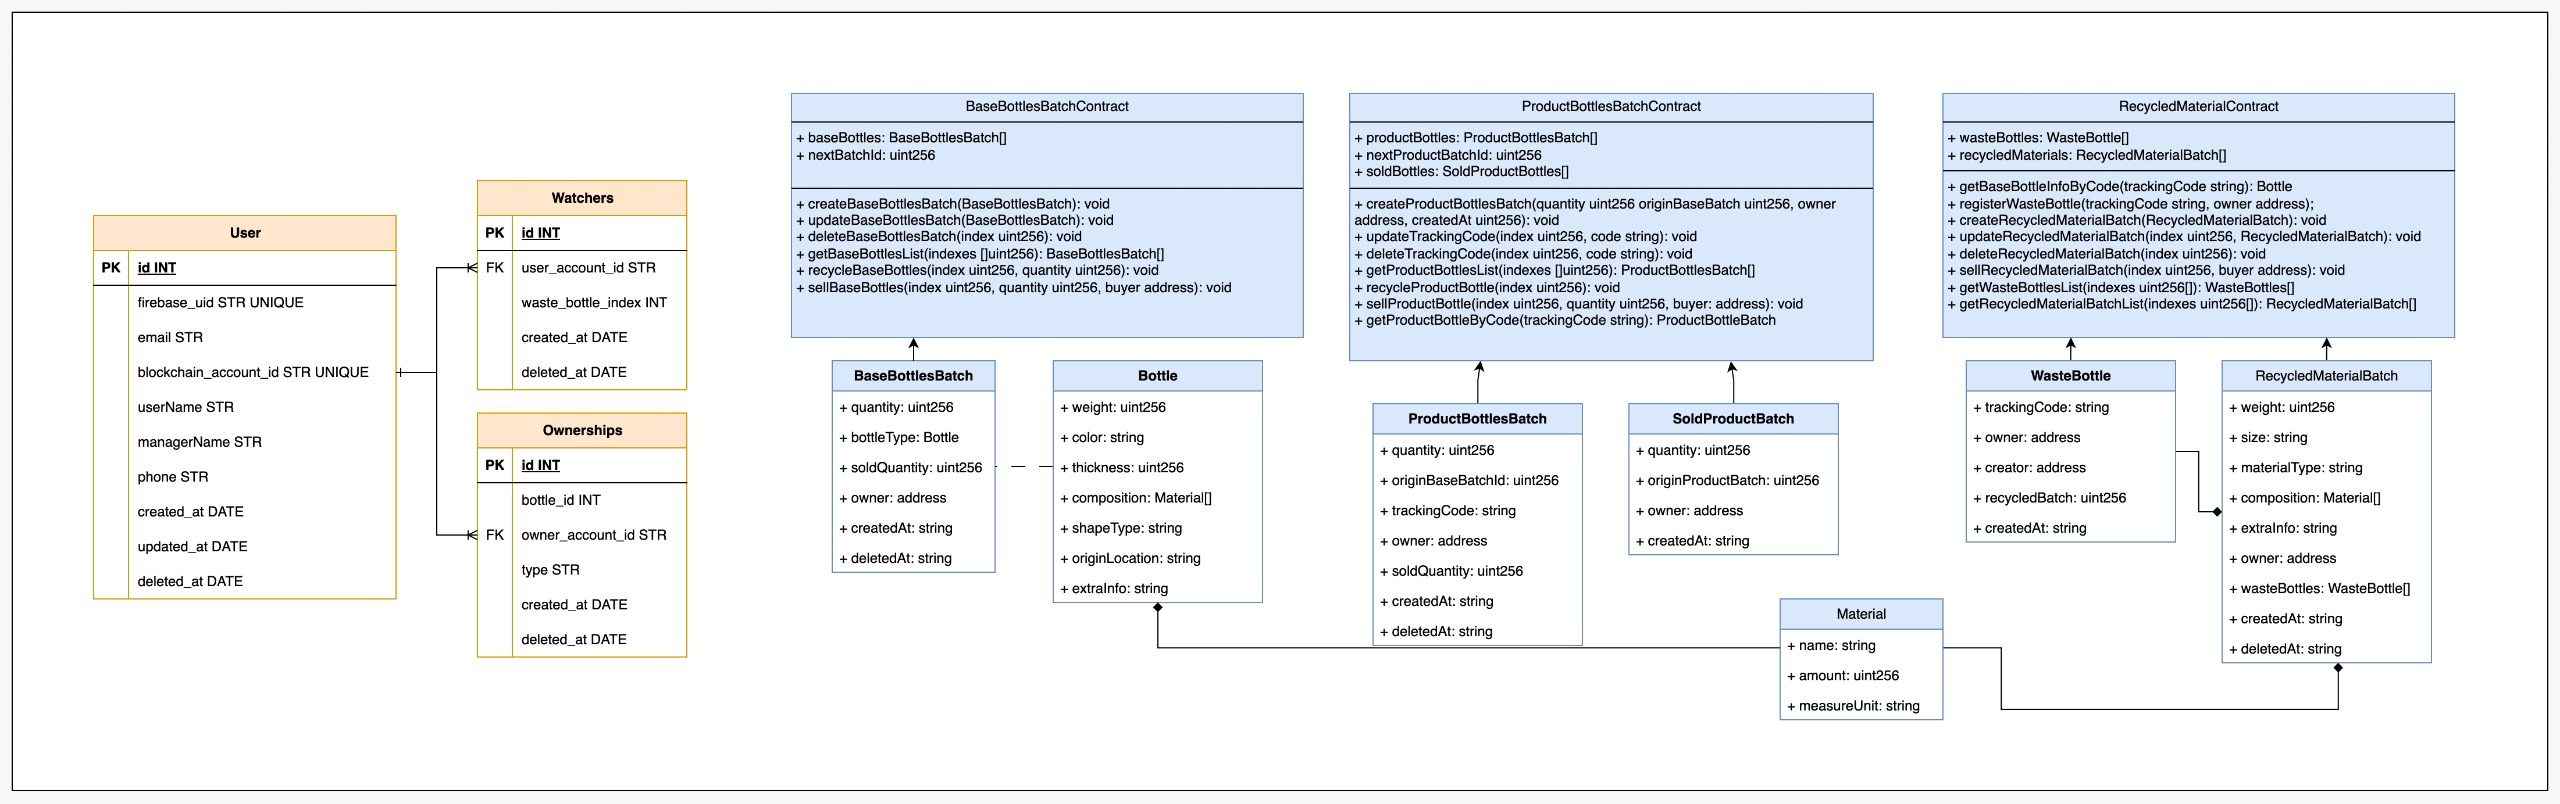
\includegraphics[width=0.8\textwidth]{Figures/database-der.jpeg}
    \caption{Diagrama Entidad-Relación (DER) del modelo de datos.}
    \label{fig:erd}
\end{figure}

Para orquestar la comunicación entre la API, la base de datos SQL y la blockchain, se implementó un patrón de diseño que unifica las operaciones de lectura y escritura. Un **_repository_** se encarga de la lógica de acceso a los datos, y un **_handler_** coordina las operaciones entre los diferentes _repositories_. Por ejemplo, para registrar un nuevo lote, el _handler_ primero valida la información y luego instruye al _repository_ de la blockchain para registrar la transacción y al _repository_ SQL para almacenar los metadatos. Este patrón abstrae la complejidad de la arquitectura híbrida, ofreciendo una interfaz de programación unificada a la capa de lógica de negocio.

---

La culminación de la etapa de diseño, con las especificaciones detalladas de la arquitectura de componentes, da paso a la siguiente fase del trabajo: la implementación. Al contar con un plan claro que define la estructura del sistema, sus módulos, sus componentes y sus interacciones, el proceso de desarrollo se vuelve más fluido y organizado, ya que se dispone de una guía precisa para la construcción de la solución. El siguiente capítulo aborda el proceso de implementación, donde se materializarán los diseños aquí descritos.